\begin{Schunk}
\begin{Sinput}
> library("Ham94", lib.loc = "../../../library")
\end{Sinput}
\end{Schunk}
Page 658 and forward provide examples of ARCH models.  Several utility functions are needed for these examples.
The function "arch.fitted.values" calculates the value of ht given the conditional information set YT and
a parameter vector THETA as described on page 660, [21.1.17] to [21.1.20].
\begin{Schunk}
\begin{Sinput}
> arch.fitted.values <- function(THETA, YT) {
+     alpha <- THETA[grep("alpha.*", names(THETA))]
+     beta <- THETA[grep("beta.*", names(THETA))]
+     zeta <- THETA["zeta"]
+     m <- length(alpha)
+     h <- rep(as.vector(zeta), m)
+     u <- YT$y - YT$x %*% beta
+     indices <- (m + 1):length(YT$y)
+     z <- array(0, c(length(indices), 1 + m))
+     for (tt in indices) h[tt] <- t(c(zeta, alpha)) %*% c(1, u[(tt - 
+         1):(tt - m)]^2)
+     list(u = u, h = h)
+ }
\end{Sinput}
\end{Schunk}
Function "arch.standard.errors" calculates values for standard errors according to the description on page 663,
particularly equations [21.1.25], and also using [21.1.21] for the estimate of the outer product estimate of the
information matrix.
\begin{Schunk}
\begin{Sinput}
> arch.standard.errors <- function(THETA, YT) {
+     x <- YT$x
+     y <- YT$y
+     k <- dim(x)[[2]]
+     alpha <- THETA[grep("alpha.*", names(THETA))]
+     zeta <- THETA["zeta"]
+     m <- length(alpha)
+     T <- length(y) - m
+     a <- k + 1 + m
+     fv <- arch.fitted.values(THETA, YT)
+     h <- fv$h
+     u2 <- fv$u^2
+     S <- array(0, c(a, a))
+     D <- array(0, c(a, a))
+     for (tt in (m + 1):length(y)) {
+         temp <- c(t(alpha) %*% ((u2[(tt - 1):(tt - m)] %o% rep(1, 
+             k)) * x[(tt - 1):(tt - m), ]), c(1, u[(tt - 1):(tt - 
+             m)]^2))
+         st <- (u2[tt] - h[tt])/(2 * h[tt]^2) * temp + c(u2[tt]/h[tt] * 
+             x[tt, ], rep(0, a - k))
+         S <- S + 1/T * st %*% t(st)
+         D <- D + 1/T * (1/(2 * h[tt]^2) * temp %*% t(temp) + 
+             rbind(cbind(1/h[tt] * x[tt, ] %*% t(x[tt, ]), array(0, 
+                 c(k, a - k))), array(0, c(a - k, a))))
+     }
+     diag(1/T * solve(D) %*% S %*% solve(D))^0.5
+ }
\end{Sinput}
\end{Schunk}
The following two helper functions calculate the likelihood values under different distributional assumptions.
The normal likelihood is calculated according to [21.1.20], the scaled t according to [21.1.24].
\begin{Schunk}
\begin{Sinput}
> arch.normal <- function(THETA, YT) {
+     fv <- arch.fitted.values(THETA, YT)
+     m <- length(THETA[grep("alpha.*", names(THETA))])
+     h <- fv$h[-1:-m]
+     u <- fv$u[-1:-m]
+     -1/2 * (length(h) * log(2 * pi) - sum(log(h)) - sum(u^2/h))
+ }
> arch.scaled.t <- function(THETA, YT) {
+     fv <- arch.fitted.values(THETA, YT)
+     m <- length(THETA[grep("alpha.*", names(THETA))])
+     h <- fv$h[-1:-m]
+     u <- fv$u[-1:-m]
+     nu <- THETA[grep("nu", names(THETA))]
+     result <- length(h) * log(gamma((nu + 1)/2)/(sqrt(pi) * gamma(nu/2)) * 
+         (nu - 2)^-0.5) - 1/2 * sum(log(h)) - (nu + 1)/2 * sum(log(1 + 
+         u^2/(h * (nu - 2))))
+ }
\end{Sinput}
\end{Schunk}
GMM estimates are calculated according to the recipe in Chapter 14, notably
equations [14.1.7] and [14.1.10].  Functions h and S are specified
by the caller.
\begin{Schunk}
\begin{Sinput}
> GMM.estimates <- function(YT, h, THETA, S) {
+     g <- function(YT, THETA) {
+         apply(X = apply(X = YT, MARGIN = 1, FUN = h, THETA = THETA), 
+             MARGIN = 1, FUN = mean)
+     }
+     objective <- function(THETA, YT, W) {
+         g.value <- g(YT, THETA)
+         as.numeric(t(g.value) %*% W %*% g.value)
+     }
+     r <- length(h(YT[1, ], THETA))
+     a <- length(THETA)
+     stage.1.results <- optim(par = THETA, fn = objective, gr = NULL, 
+         YT = YT, W = diag(r))
+     temp <- t(apply(X = YT, MARGIN = 1, FUN = h, THETA = stage.1.results$par))
+     ST <- S(temp)
+     stage.2.results <- optim(par = stage.1.results$par, fn = objective, 
+         gr = NULL, YT = YT, W = solve(ST))
+     list(stage.1.results = stage.1.results, stage.2.results = stage.2.results)
+ }
\end{Sinput}
\end{Schunk}
\subsection{Application of ARCH Models to US Fed Funds Data}
The dataset for these examples is the US Fed Funds Rate, monthly between Jan 1955 and December 2000,
shown below.
\begin{Schunk}
\begin{Sinput}
> data(fedfunds, package = "Ham94")
> selection <- subset(fedfunds, Month >= "1955-01-01" & Month <= 
+     "2000-12-01")
> y <- selection$FFED
\end{Sinput}
\end{Schunk}
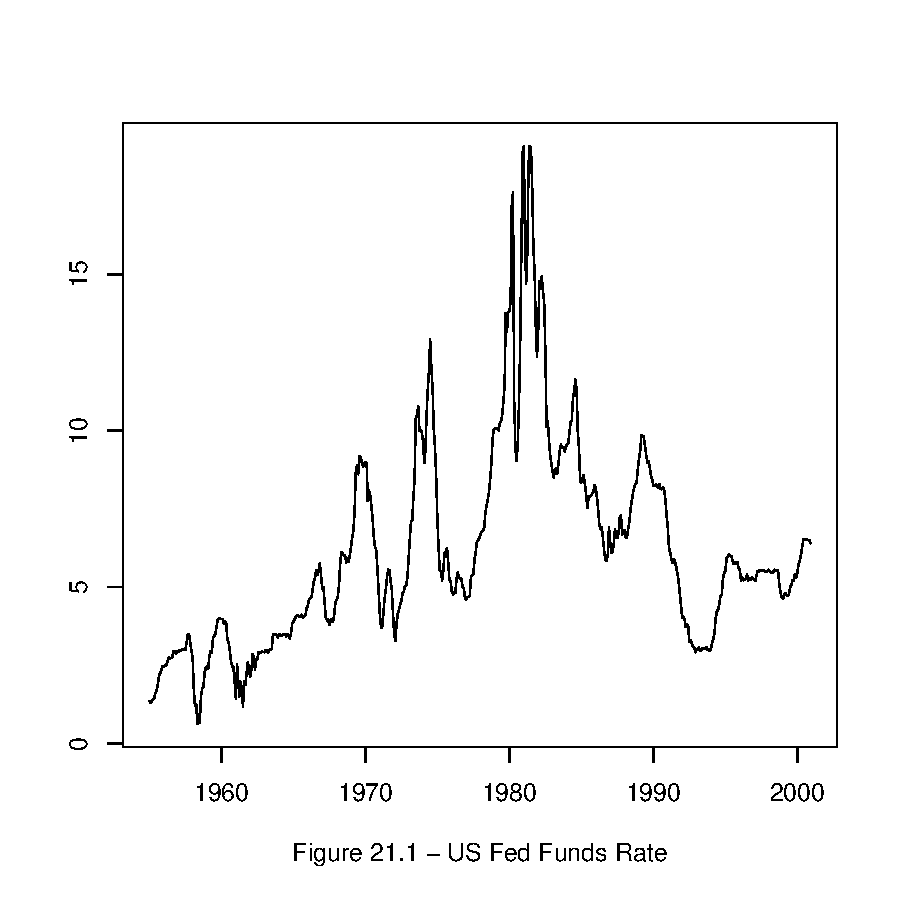
\includegraphics{p660-007}
A first step is to characterize the autocorrelation structure of the squared residuals.  These two regressions
show that a second order AR process seems to fit the data pretty well.
\begin{Schunk}
\begin{Sinput}
> y.lm <- lm(y ~ 1 + y_1, list(y = y[-1], y_1 = y[-length(y)]))
> u <- y.lm$residuals
> u2.lm <- lm(u2 ~ 1 + u2_lag, list(u2 = u[-1:-4]^2, u2_lag = embed(u[-length(u)]^2, 
+     4)))
> F34 <- Wald.F.Test(R = cbind(rep(0, 2) %o% rep(0, 3), diag(2)), 
+     b = u2.lm$coefficients, r = c(0, 0), s2 = summary(u2.lm)$sigma^2, 
+     XtX_1 = summary(u2.lm)$cov.unscaled)
> F34.sig <- 1 - pf(F34, 2, length(u2.lm$residuals) - u2.lm$rank)
> F234 <- Wald.F.Test(R = cbind(rep(0, 3) %o% rep(0, 2), diag(3)), 
+     b = u2.lm$coefficients, r = c(0, 0, 0), s2 = summary(u2.lm)$sigma^2, 
+     XtX_1 = summary(u2.lm)$cov.unscaled)
> F234.sig <- 1 - pf(F234, 3, length(u2.lm$residuals) - u2.lm$rank)
> accept.arch <- pchisq(length(u2.lm$residuals) * summary(u2.lm)$r.squared, 
+     4)
> print(F34)
\end{Sinput}
\begin{Soutput}
[1] 0.8225742
\end{Soutput}
\begin{Sinput}
> print(F34.sig)
\end{Sinput}
\begin{Soutput}
[1] 0.439847
\end{Soutput}
\begin{Sinput}
> print(F234)
\end{Sinput}
\begin{Soutput}
[1] 11.88167
\end{Soutput}
\begin{Sinput}
> print(F234.sig)
\end{Sinput}
\begin{Soutput}
[1] 1.513714e-07
\end{Soutput}
\begin{Sinput}
> print(accept.arch)
\end{Sinput}
\begin{Soutput}
[1] 1
\end{Soutput}
\end{Schunk}
Next we use a maximum likelihood estimation to estimate the parameters for the second
order equation assuming normal errors.
\begin{Schunk}
\begin{Sinput}
> YT <- list(y = y[-1], x = cbind(rep(1, length(y) - 1), y[-length(y)]))
> THETA <- c(beta = y.lm$coefficients, zeta = var(y.lm$residuals), 
+     alpha = c(0.1, 0.1))
> optimizer.results <- optim(par = THETA, fn = arch.normal, gr = NULL, 
+     YT = YT)
> print(optimizer.results$par)
\end{Sinput}
\begin{Soutput}
beta.(Intercept)         beta.y_1             zeta           alpha1 
      0.25226382       0.94858488       0.02734929       0.95530391 
          alpha2 
      0.29858866 
\end{Soutput}
\begin{Sinput}
> se <- arch.standard.errors(optimizer.results$par, YT)
> print(se)
\end{Sinput}
\begin{Soutput}
[1] 0.048395622 0.010418563 0.004969357 0.108784800 0.082012310
\end{Soutput}
\end{Schunk}
Now use GMM to estimate the same parameters following page 664.  The initial values
for the regression coefficients are derived from the (homoskedastic) regression above,
as is the presample variance.  The estimator for S assumes no correlation at leads and lags.
\begin{Schunk}
\begin{Sinput}
> h <- function(wt, THETA) {
+     beta <- THETA[grep("beta.*", names(THETA))]
+     zeta <- THETA["zeta"]
+     alpha <- THETA[grep("alpha.*", names(THETA))]
+     m <- length(alpha)
+     k <- length(beta)
+     yt <- wt[grep("yt.*", names(wt))]
+     xt <- wt[grep("xt.*", names(wt))]
+     ylagt <- wt[grep("ylagt.*", names(wt))]
+     xlagt <- t(array(wt[grep("xlagt.*", names(wt))], c(k, m)))
+     ut <- yt - t(xt) %*% beta
+     zt <- c(1, (ylagt - t(xlagt) %*% beta)^2)
+     c(ut * xt, (ut^2 - t(zt) %*% c(zeta, alpha)) * zt)
+ }
> S.estimator <- function(ht) {
+     1/dim(ht)[[1]] * t(ht) %*% ht
+ }
> THETA <- c(beta = y.lm$coefficients, zeta = var(y.lm$residuals), 
+     alpha = c(0.1, 0.1))
> m <- length(THETA[grep("alpha.*", names(THETA))])
> T <- length(YT$y) - m
> w <- as.matrix(data.frame(yt = YT$y[-1:-m], xt = YT$x[-1:-m, 
+     ], ylagt = embed(YT$y[-(T + m)], m), xlagt = embed(YT$x[-(T + 
+     m), ], m)))
> estimates <- GMM.estimates(YT = w, h = h, THETA = THETA, S.estimator)
> print(estimates$stage.1.results$par)
\end{Sinput}
\begin{Soutput}
beta.(Intercept)         beta.y_1             zeta           alpha1 
      0.05788674       0.98955937       0.32491651       0.01073606 
          alpha2 
      0.02105476 
\end{Soutput}
\begin{Sinput}
> print(estimates$stage.2.results$par)
\end{Sinput}
\begin{Soutput}
beta.(Intercept)         beta.y_1             zeta           alpha1 
      0.02579794       0.99791508      -0.17911928       0.01239927 
          alpha2 
      0.07770754 
\end{Soutput}
\end{Schunk}
\subsection{R Facilities For GARCH models}
TBD
